\chapter{Robots}
	\index{robot}
    \index{robotics}
    \label{chap:Robots}
        In this chapter I will list several robots used in both the Nationals performance, and other robots developed for \index{regionals}regionals and \index{state}state performances.
    
    	\section{BaralabaBob}
        	\label{sec:BaralabaBob}
    		BaralabaBob is the main piece of the show, being a 6-legged Lynxmotion APod.\\
    		
    		\subsection{Technical Manual}
    			A seperate document, \hyperref[part:part_six]{BaralabaBob Technical Manual}, has been created, and it contains all the relevant information.
    		
    		\subsection{Construction}
    			\index{BaralabaBob}BaralabaBob first arrived on October 18th, 2014. Construction began, and took 6 days to assemble the mechanicals, and write the base \index{python}python code, of which he still uses parts of to this day.
    			
    
    			\centerline{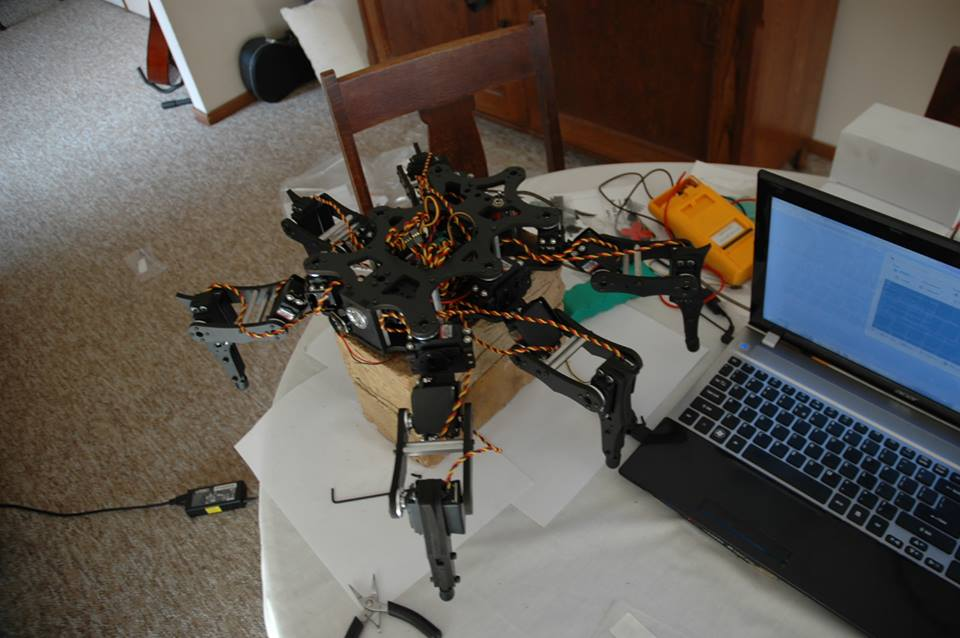
\includegraphics[width=\linewidth]{images/apod_build3}}
    			\centerline{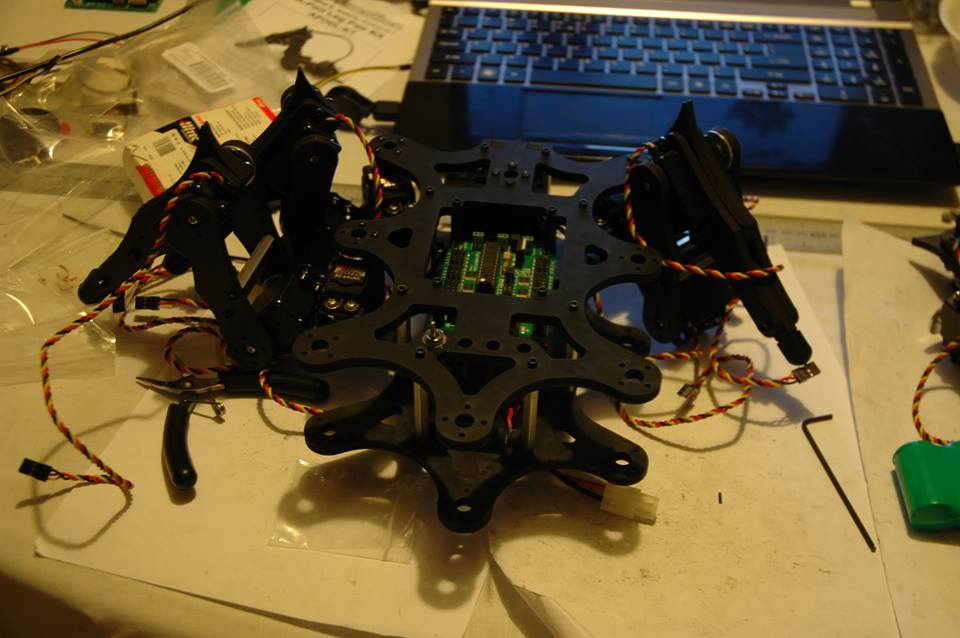
\includegraphics[width=\linewidth]{images/apod_build2}}
    			\centerline{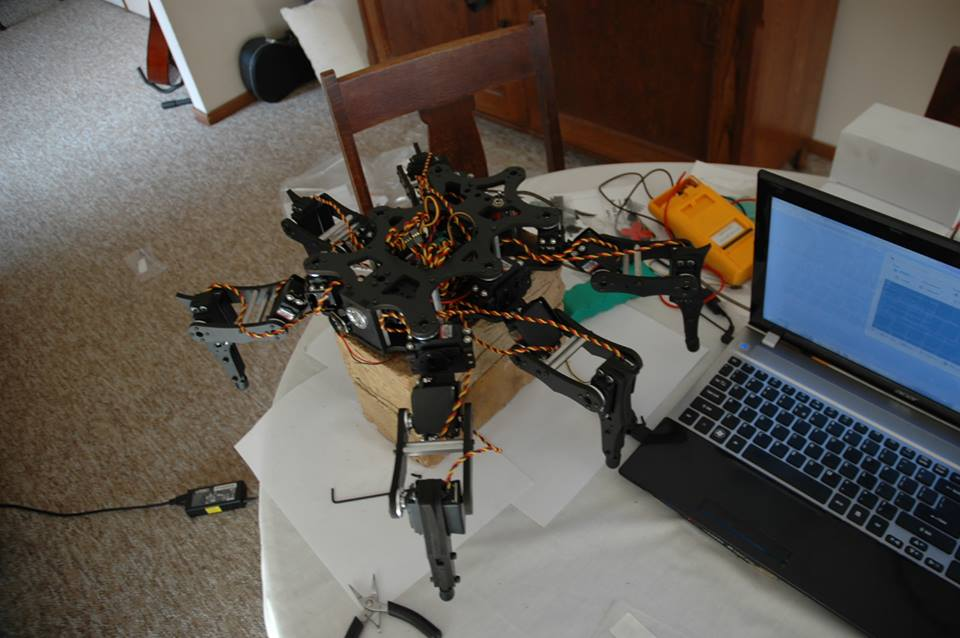
\includegraphics[width=\linewidth]{images/apod_build3}}
    			\centerline{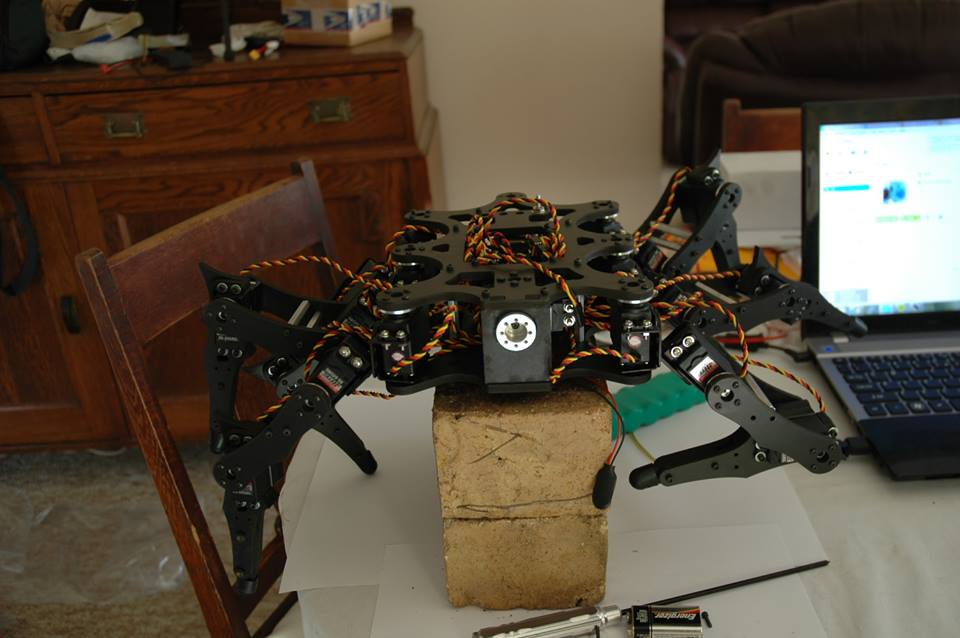
\includegraphics[width=\linewidth]{images/apod_build4}}
    			\centerline{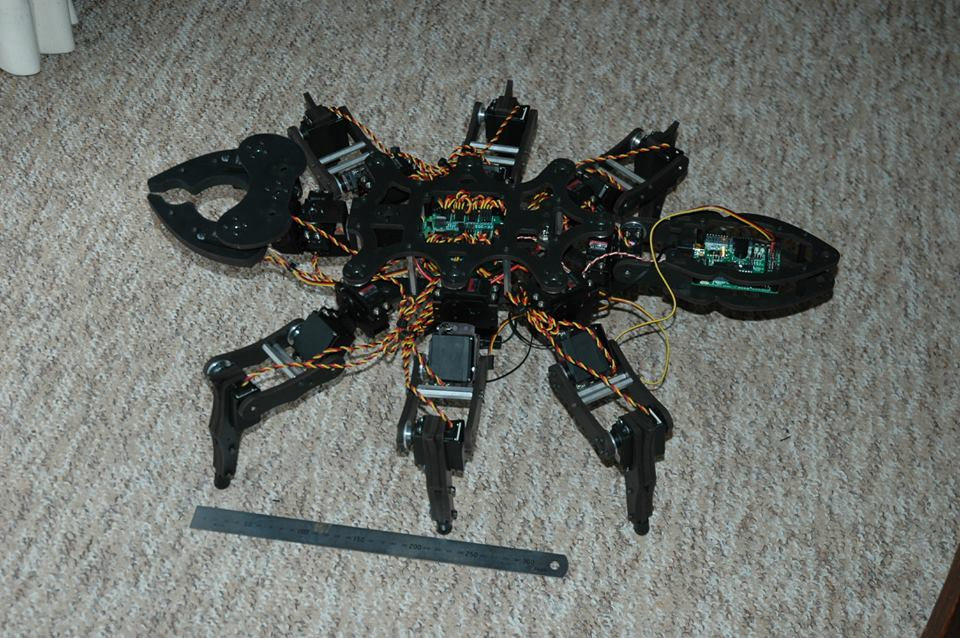
\includegraphics[width=\linewidth]{images/apod_build5}}
    			\centerline{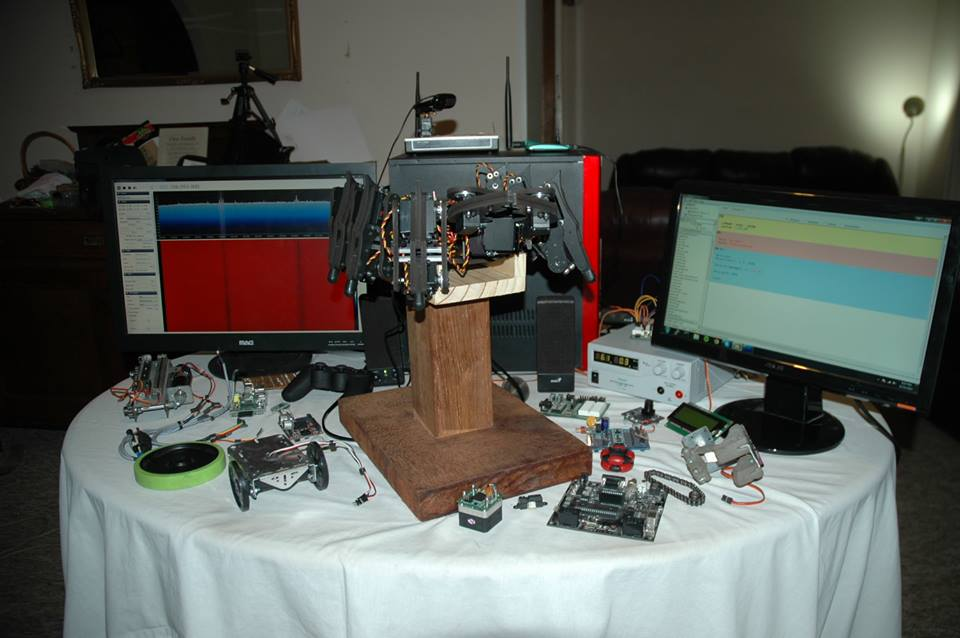
\includegraphics[width=\linewidth]{images/apod_build6}}
    			
    		\subsection{Software}
    			Consult \hyperref[part:part_six]{BaralabaBob Technical Manual} for more information.
    			
    			\pagebreak
    
    \label{sec:BobMobile}
    \label{sec:Beaker}
    \section{BobMobile}
    	\index{Beaker}\index{BobMobile}BobMobile is the robot that BaralabaBob rides out in the first part of the performance.
    	
    	\subsection{History}
    		Whilst living in \index{Baralaba}Baralaba, John became known to some locals as the "robotics guy". One of these particular people was good enough to give us some spare \index{motors}motors out of an electric car seat that he didn't need.\\
    		
    		The motors were quite good as they had a good speed for a mobile base, as well as having good torque. However their axle had worm drive on it. I took it to a local engineering firm, who kindly agreed mill the teeth of the motor axles.\\
    		
    		After having brackets built for the motors, John mounted the motors on a small wooden base. His intention was to use this base for general experimentation with bulkier systems, such as \index{laser scanner}laser scanners and \index{computer vision}Computer Vision using a laptop. This robot's name was \index{Beaker}Beaker. \\
    		
    		\centerline{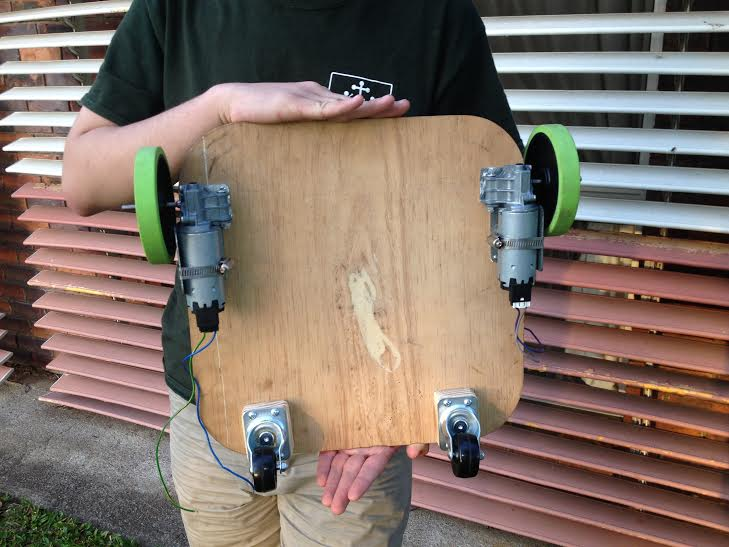
\includegraphics[width=0.75\linewidth]{images/beaker_bottom}}
    		\centerline{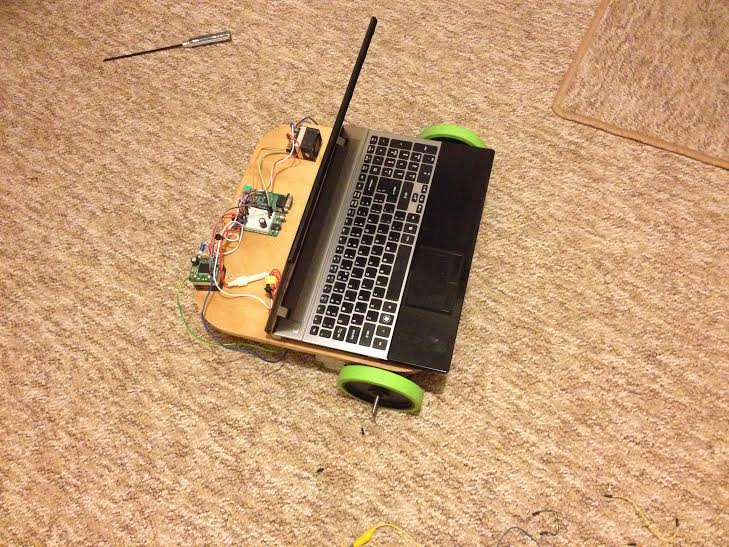
\includegraphics[width=0.75\linewidth]{images/beaker_top}}
    		
    		As I've talked about in the \index{Goombungee}\hyperref[chap:history]{Goombungee Show chapter}, Beaker was used as an interactive \index{exhibit} - being integrated with the \index{HID}HID devices of a \index{joystick}Joystick, and the \index{Microsoft}Microsoft \index{Kinect}Kinect.\\
    		
    		I wished to have \index{BaralabaBob}BaralabaBob ride out on Beaker for RCJA QLD State Championships. Beaker was too small for the \index{hexapod}hexapod to fit on, so I widened the base, and added a second deck. At this point it's name changed to \index{BobMobile}\index{Beaker}BobMobile.\\
    		
    	\subsection{Controllers}
    		Originally \index{BaralabaBob}BaralabaBob shipped with Lynxmotion's \hyperlink{http://www.lynxmotion.com/c-153-botboarduino.aspx}{BotBoarduino}. I soon replaced that with a \hyperref[RPi]{RaspberryPi}, but decided the \hyperref[BotBoarduino]{BotBoarduino} would be good for the BobMobile.\\
            
            \textit{\textbf{Also see:}\hyperref[Controllers]{Controllers}}
    		
    		The motor controllers are the HB-25 motor controllers from Parallax Inc.\\
    		
    		Find below a picture of when I made a mistake when soldering the powersystem on Veroboard. The whole copper track burnt(?) and peeled away from the PCB.\\
    		
    		\centerline{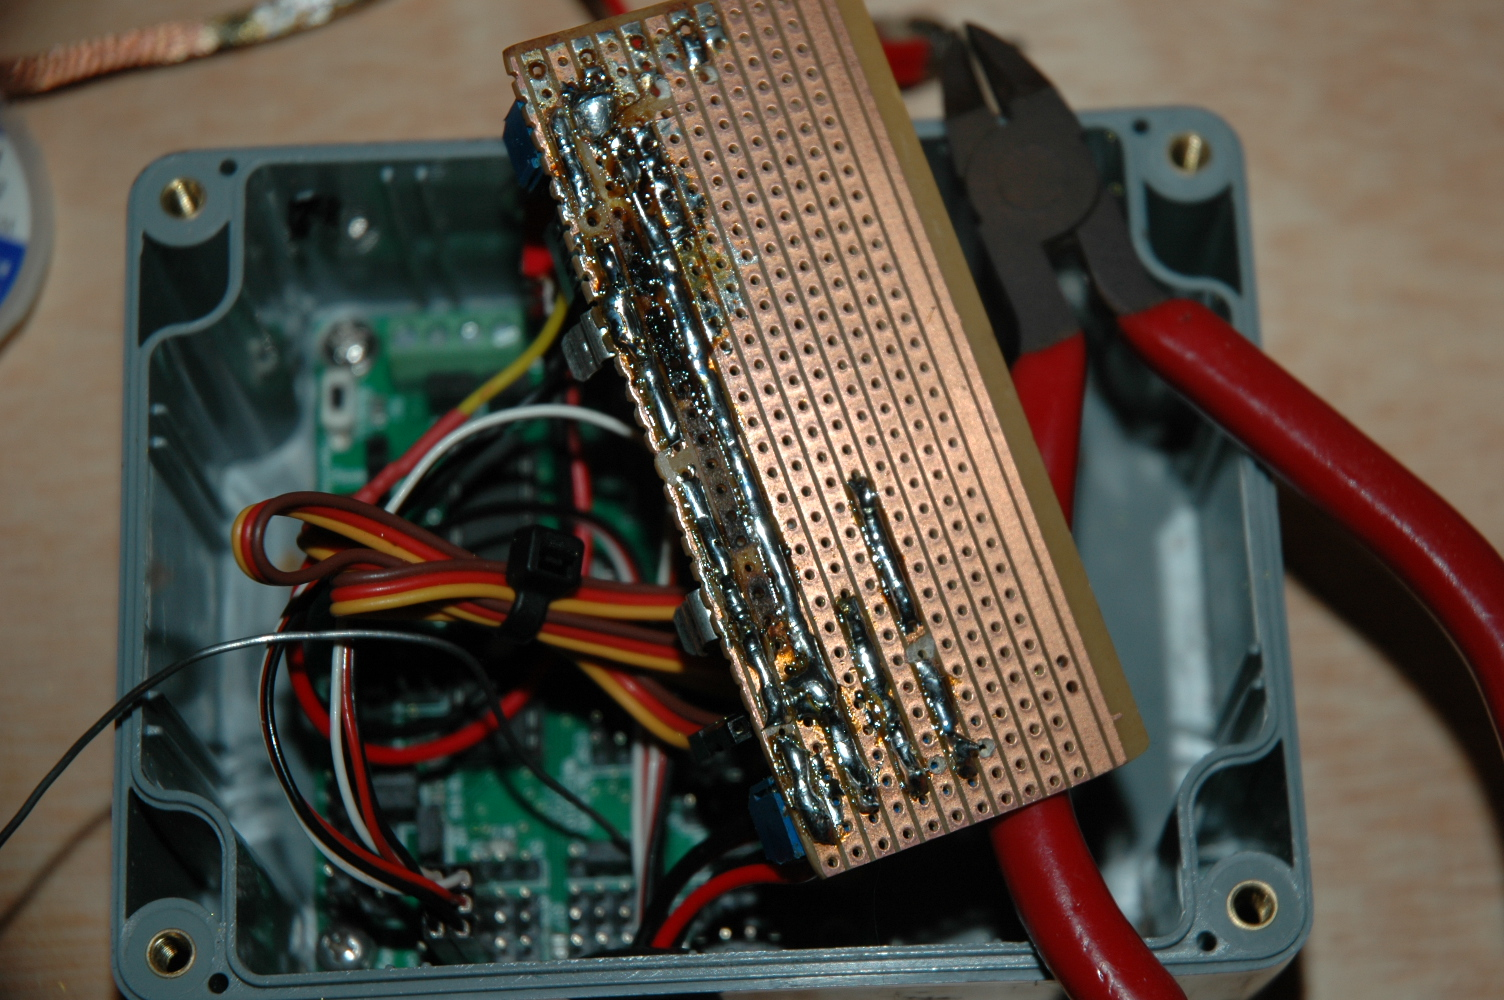
\includegraphics[width=0.75\linewidth]{images/PeelyPCB}}
    		
    	\subsection{Software}
    		\subsubsection{Beaker}
            \index{beaker}
    			All software for Beaker can be found here:\\
    			
    			\url{https://github.com/boar401s2/Beaker}
    			
    			This software includes \index{joystick}joystick and should include \index{Kinect}Kinect code. It was mainly used for the \index{Goombungee}Goombungee Exhibit. The code is written in a variety of \index{languages}languages including \index{python}Python, Bash, \index{C\#}C\#, \index{SPIN}SPIN, and SPASM (SPIN Assembly).\\
    			
    		\subsubsection{BobMobile}
    			The BobMobile code can be found here:\\
    			
    			\url{https://github.com/boar401s2/BobMobile}
    			
    			This is the software used for the competition. The code is written in \index{arduino}Arduino.\\
    	
    	\subsection{Decks}
    		\subsubsection{Bottom Deck}
            	\index{deck}
    			The bottom deck is for the \index{hexapod}hexapod to stand on.\\
    			
    		\subsubsection{Top Deck}
    			The top deck was made in anticipation for future expansion to using the \hyperref[laser_localization]{Laser Localization System}, and \hyperref[helicopter_system]{Helicopter Systems} outlined in the \hyperref[RandD]{Research and Development} chapter.\\
    			
    			\centerline{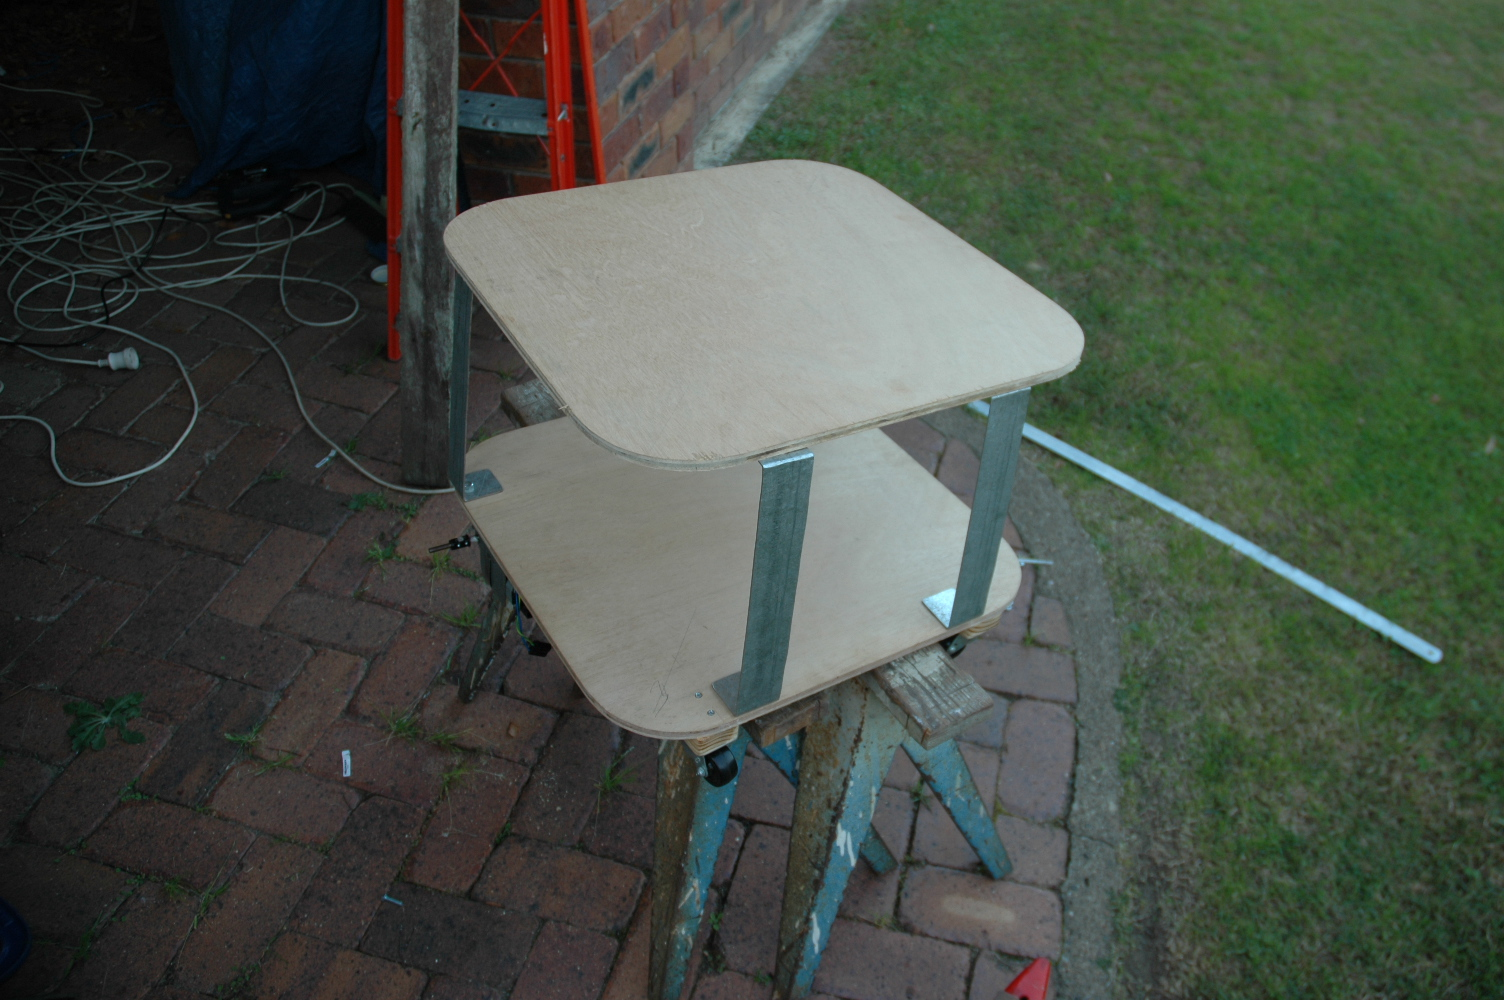
\includegraphics[width=0.75\linewidth]{images/SecondDeck}}
    		
	\label{sec:Stage}            
    \section{Stage}
    	\index{stage}
    	The "stage" is the PVC frame with black covering, and red curtains used in the RCJA QLD State Championships, 2015.
    	
    	\subsection{Sub-systems}
    		The Stage as a whole has several systems linked together - the Fog, the Lights, the Curtains, and the Button-sync systems.
            
            \textit{\textbf{See Also: }\hyperref[RandD]{Research and Development}}
    		
    		\subsubsection{The Curtains}
    			The curtains are arguably the hardest part of the stage to implement - but perhaps the most spectacular.\\
    			
    			The system works on a series of pulleys and string, along with a counterweight.\\
    			
    			I didn't have time to install an \index{end stop}end stop \index{microswitch}microswitch to tell the system when the curtains were open and closed. Instead I used feedback from the current monitoring system on the \index{ESCON}\index{Maxon}ESCON 36/2 drivers from Maxon. The drivers send back a signal to me when the motors are straining, which gives me a good indication of when the curtains have reached the end of their limit.\\				
    			
    			\centerline{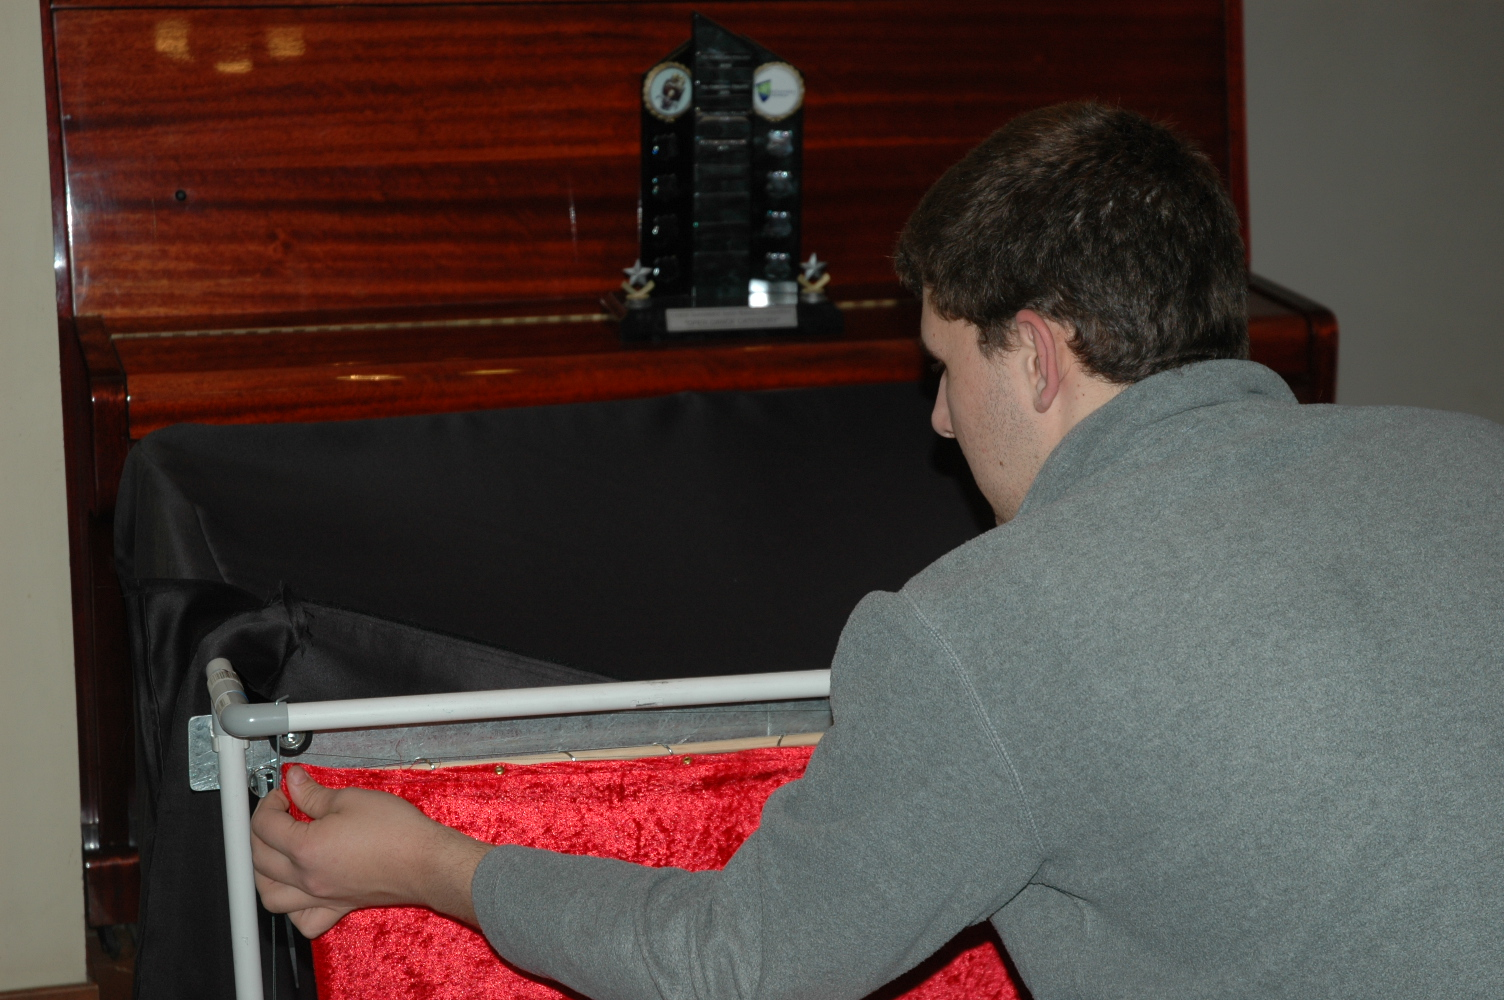
\includegraphics[width=0.75\linewidth]{images/CurtainDevelopment}}
    			
    		\subsection{The Fog}
    			See more about the fog in it's section in the \hyperref[RandD]{Research and Development} Chapter.
    			
    		\subsection{The Lighting}
    			See more about the lighting in it's section in the \hyperref[RandD]{Research and Development} chapter.
    			
    		\subsection{Button-sync}
    			Find out more about button-syncing in the lighting section in the \hyperref[RandD]{Research and Development} chapter.
    	
    	\subsection{Design Considerations}
    		I designed the whole stage with the concept of \index{portability}portability - I needed to fit it in the boot of a car, and, should the need arise, in the baggage compartment of a plane.\\
    		
    		Because of these reasons, I designed it to be collapsible, and use common \index{PVC}PVC tubing.\\
    		
    		\centerline{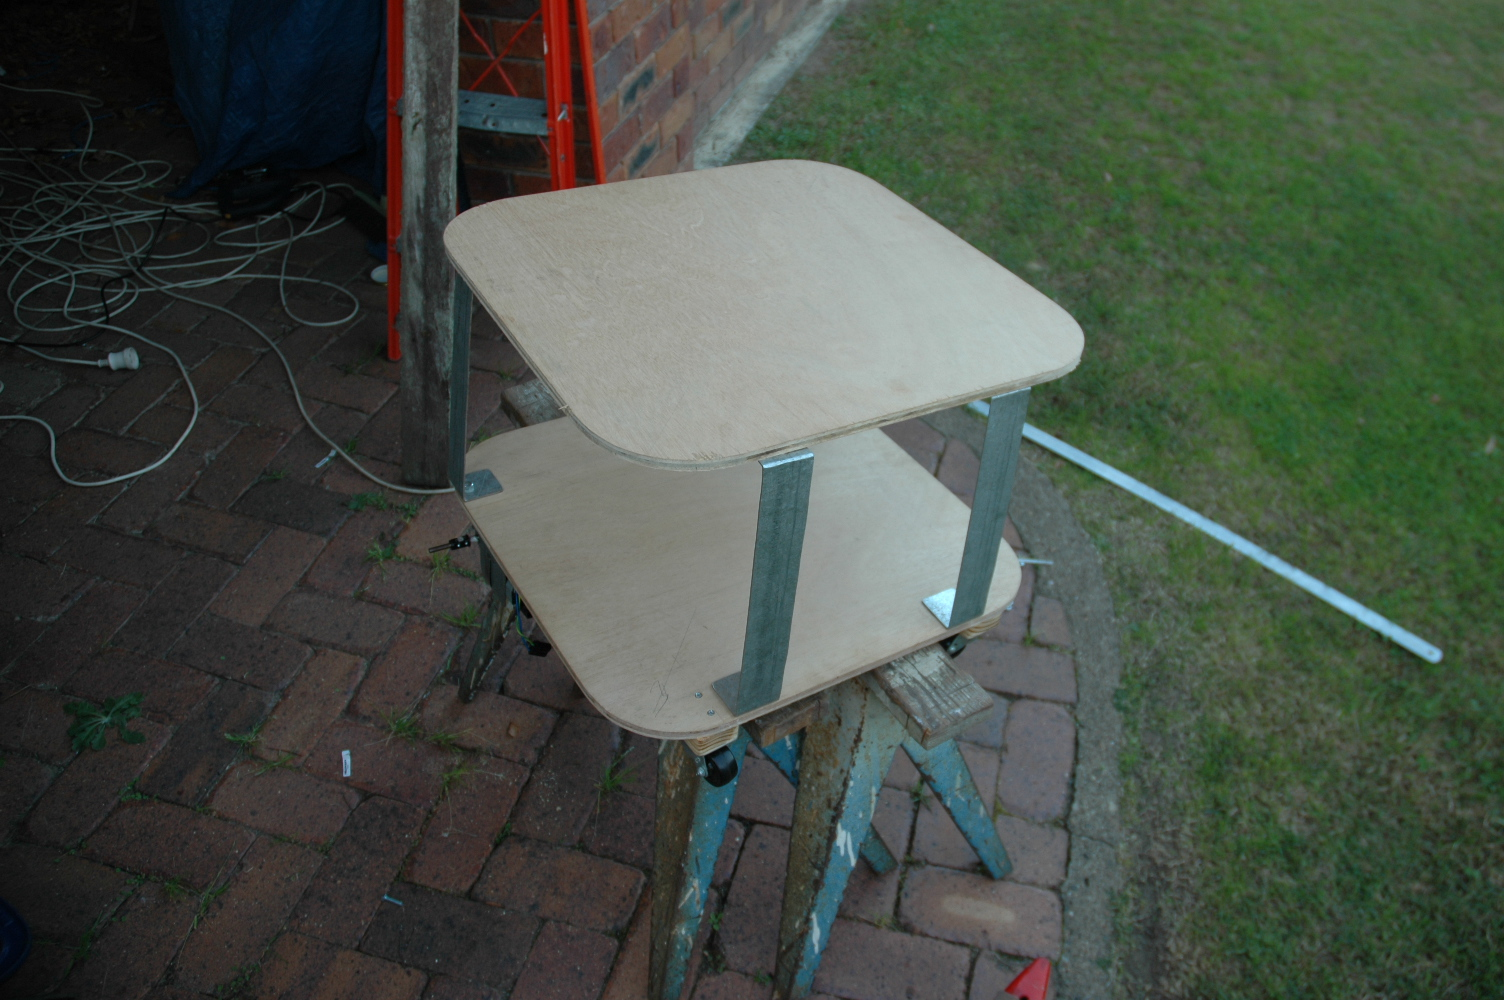
\includegraphics[width=0.75\linewidth]{images/SecondDeck}}